\clearpage
% ==============================================================================
% ==============================================================================
%                      SIMULATION ENVIRONMENT MODELING
% ==============================================================================
% ==============================================================================
\section{Simulation Environment Modeling}

Before an AI agent can learn a medical procedure, it needs a believable virtual world to practice in. Since this is a deep reinforcement learning project and not a Hollywood movie, our 3D models must strike a tricky balance: realistic enough to provide useful visual features, but simple enough to run at high speeds without crashing the physics engine. Here, we break down the four main puzzle pieces: the endoscope, snare, colon, and polyp.

% ==============================================================================
%                              ENDOSCOPE MODELING
% ==============================================================================
\subsection{Endoscope Modeling}

The endoscope acts as the \textbf{``eyes and hands''} of our system. Clinical endoscopes are incredible feats of engineering, packing an HD camera, illumination, and steering mechanics into a flexible tube just \textbf{9 to 13 millimetres} thick. While standard colonoscopes are up to 170\,cm long, simulating their full soft-body physics in Unity would instantly kill our frame rate and make deep reinforcement learning impossible. 

Instead, we relied on \textbf{smart abstraction}, focusing purely on the functional bits that shape the agent's observation and action spaces. Figure~\ref{fig:model_endoscope_full} shows our 3D models.

\begin{figure}[H]
\centering
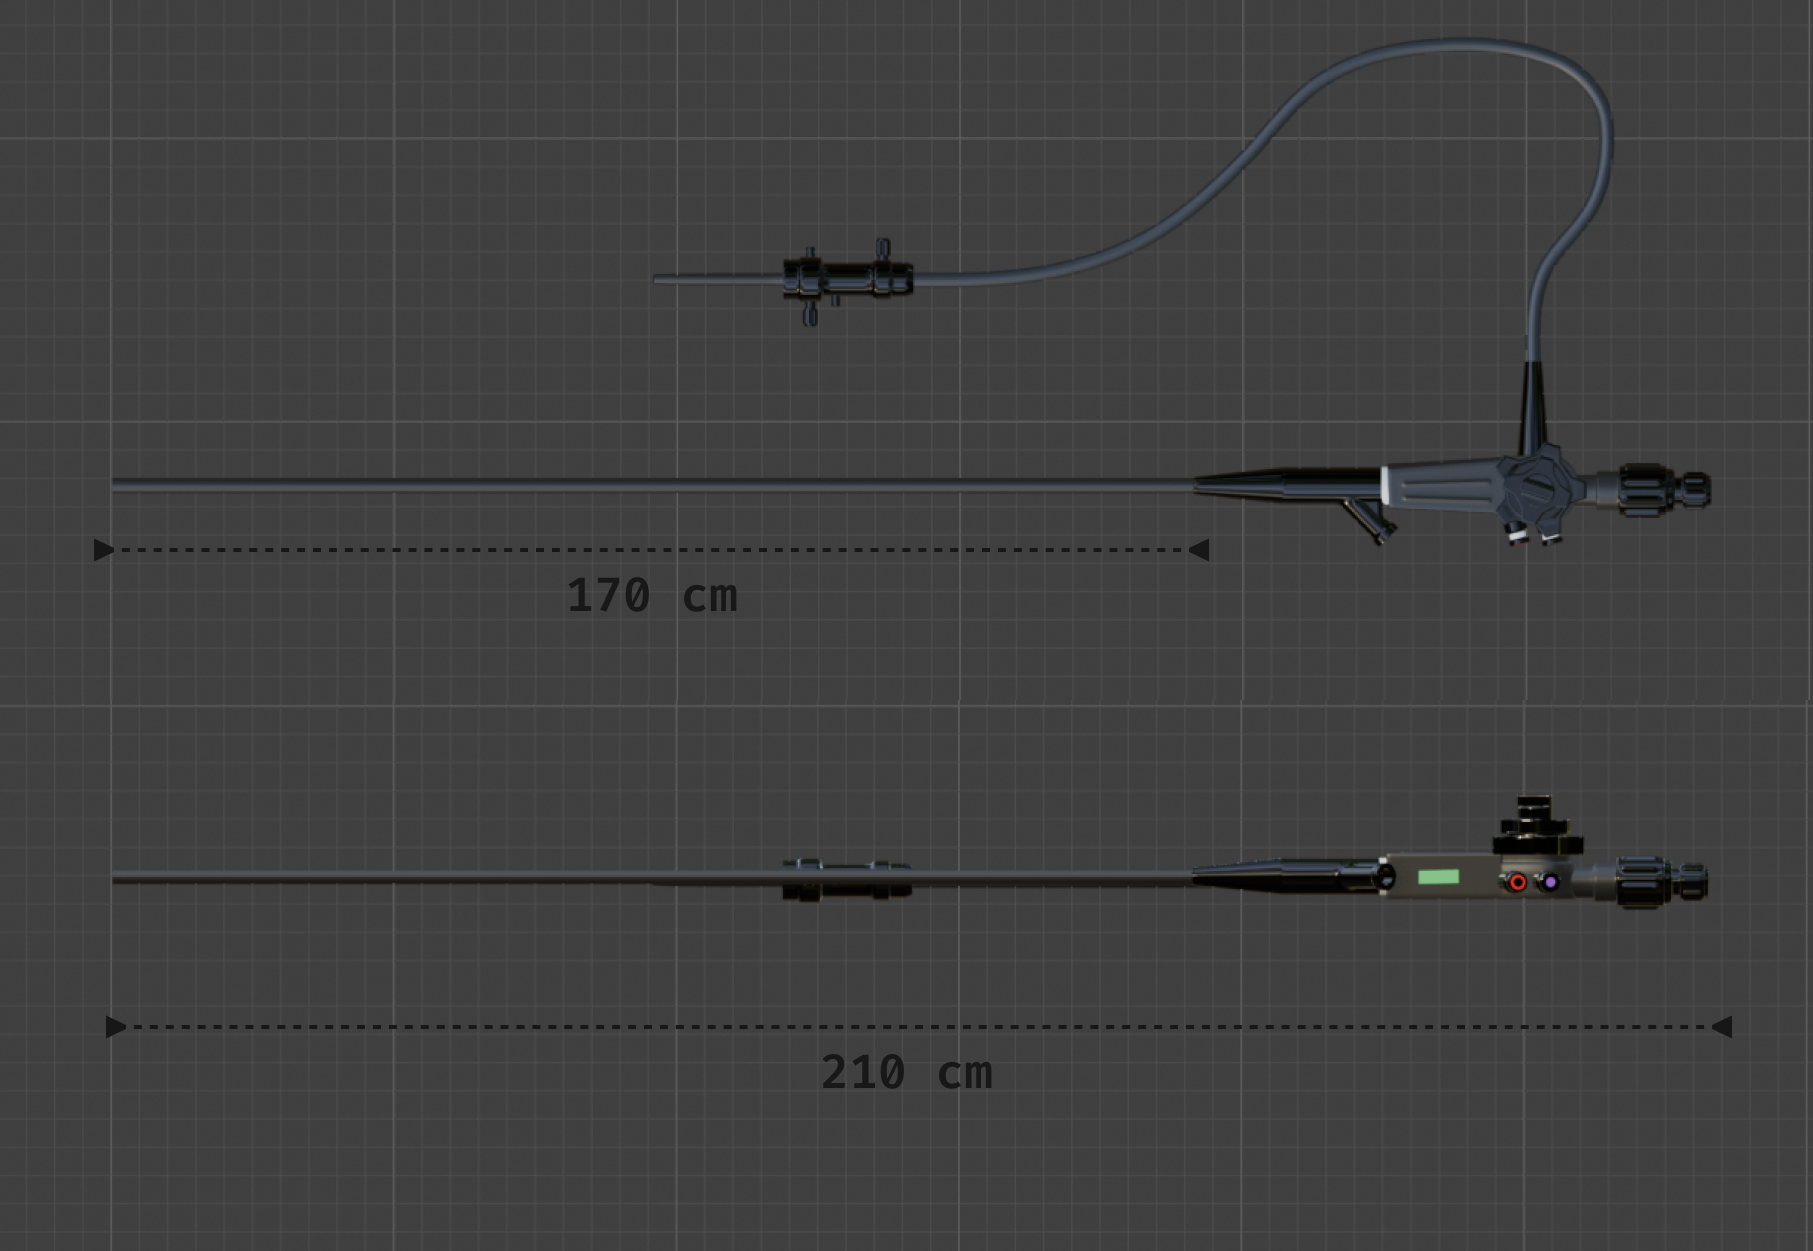
\includegraphics[width=0.6\linewidth]{assets/model-Endo Dim 1.png}
\caption{Full-length 3D renders of our endoscope model (170\,cm).}
\label{fig:model_endoscope_full}
\end{figure}

\paragraph{Distal tip isolation and steering.}
The agent only controls the \textbf{distal tip}, modeled as a \textbf{rigid cylinder} on an \textbf{articulated kinematic joint} mimicking a flexible \textbf{bending section}. Rotational \textbf{pitch} and \textbf{yaw} are capped at \textbf{160 degrees}, and steered via smoothed \textbf{controlled torques}. Figure~\ref{fig:model_endoscope_head} details the physical control head.

In a physical clinical setting, this angulation is achieved via two \textbf{nested control knobs} manipulated by the physician's thumb. These dials pull on internal \textbf{Bowden cables} (steering wires) running the entire 170\,cm length of the insertion tube, culminating in the bending section. This mechanical linkage introduces a ton of \textbf{hysteresis, friction, and nonlinear responsiveness}, which doctors commonly call \textbf{``whip'' or ``backlash.''} By abstracting this intricate mechanical reality into a \textbf{kinematic joint} steered via direct torques, we bypass the computationally devastating task of simulating cable friction. Consequently, our agent learns an \textbf{idealized, instantaneous mapping} from visual input to tip angulation. This definitely introduces a notable \textbf{\textit{sim-to-real} gap} because the simulated endoscope feels way more responsive than a real one. However, we did this on purpose to isolate the core visual-navigation problem from the chaotic physics of mechanical cables. Future work could introduce \textbf{synthetic delay or noise} into these control signals to eventually bridge this gap for physical deployment.

\begin{figure}[H]
\centering
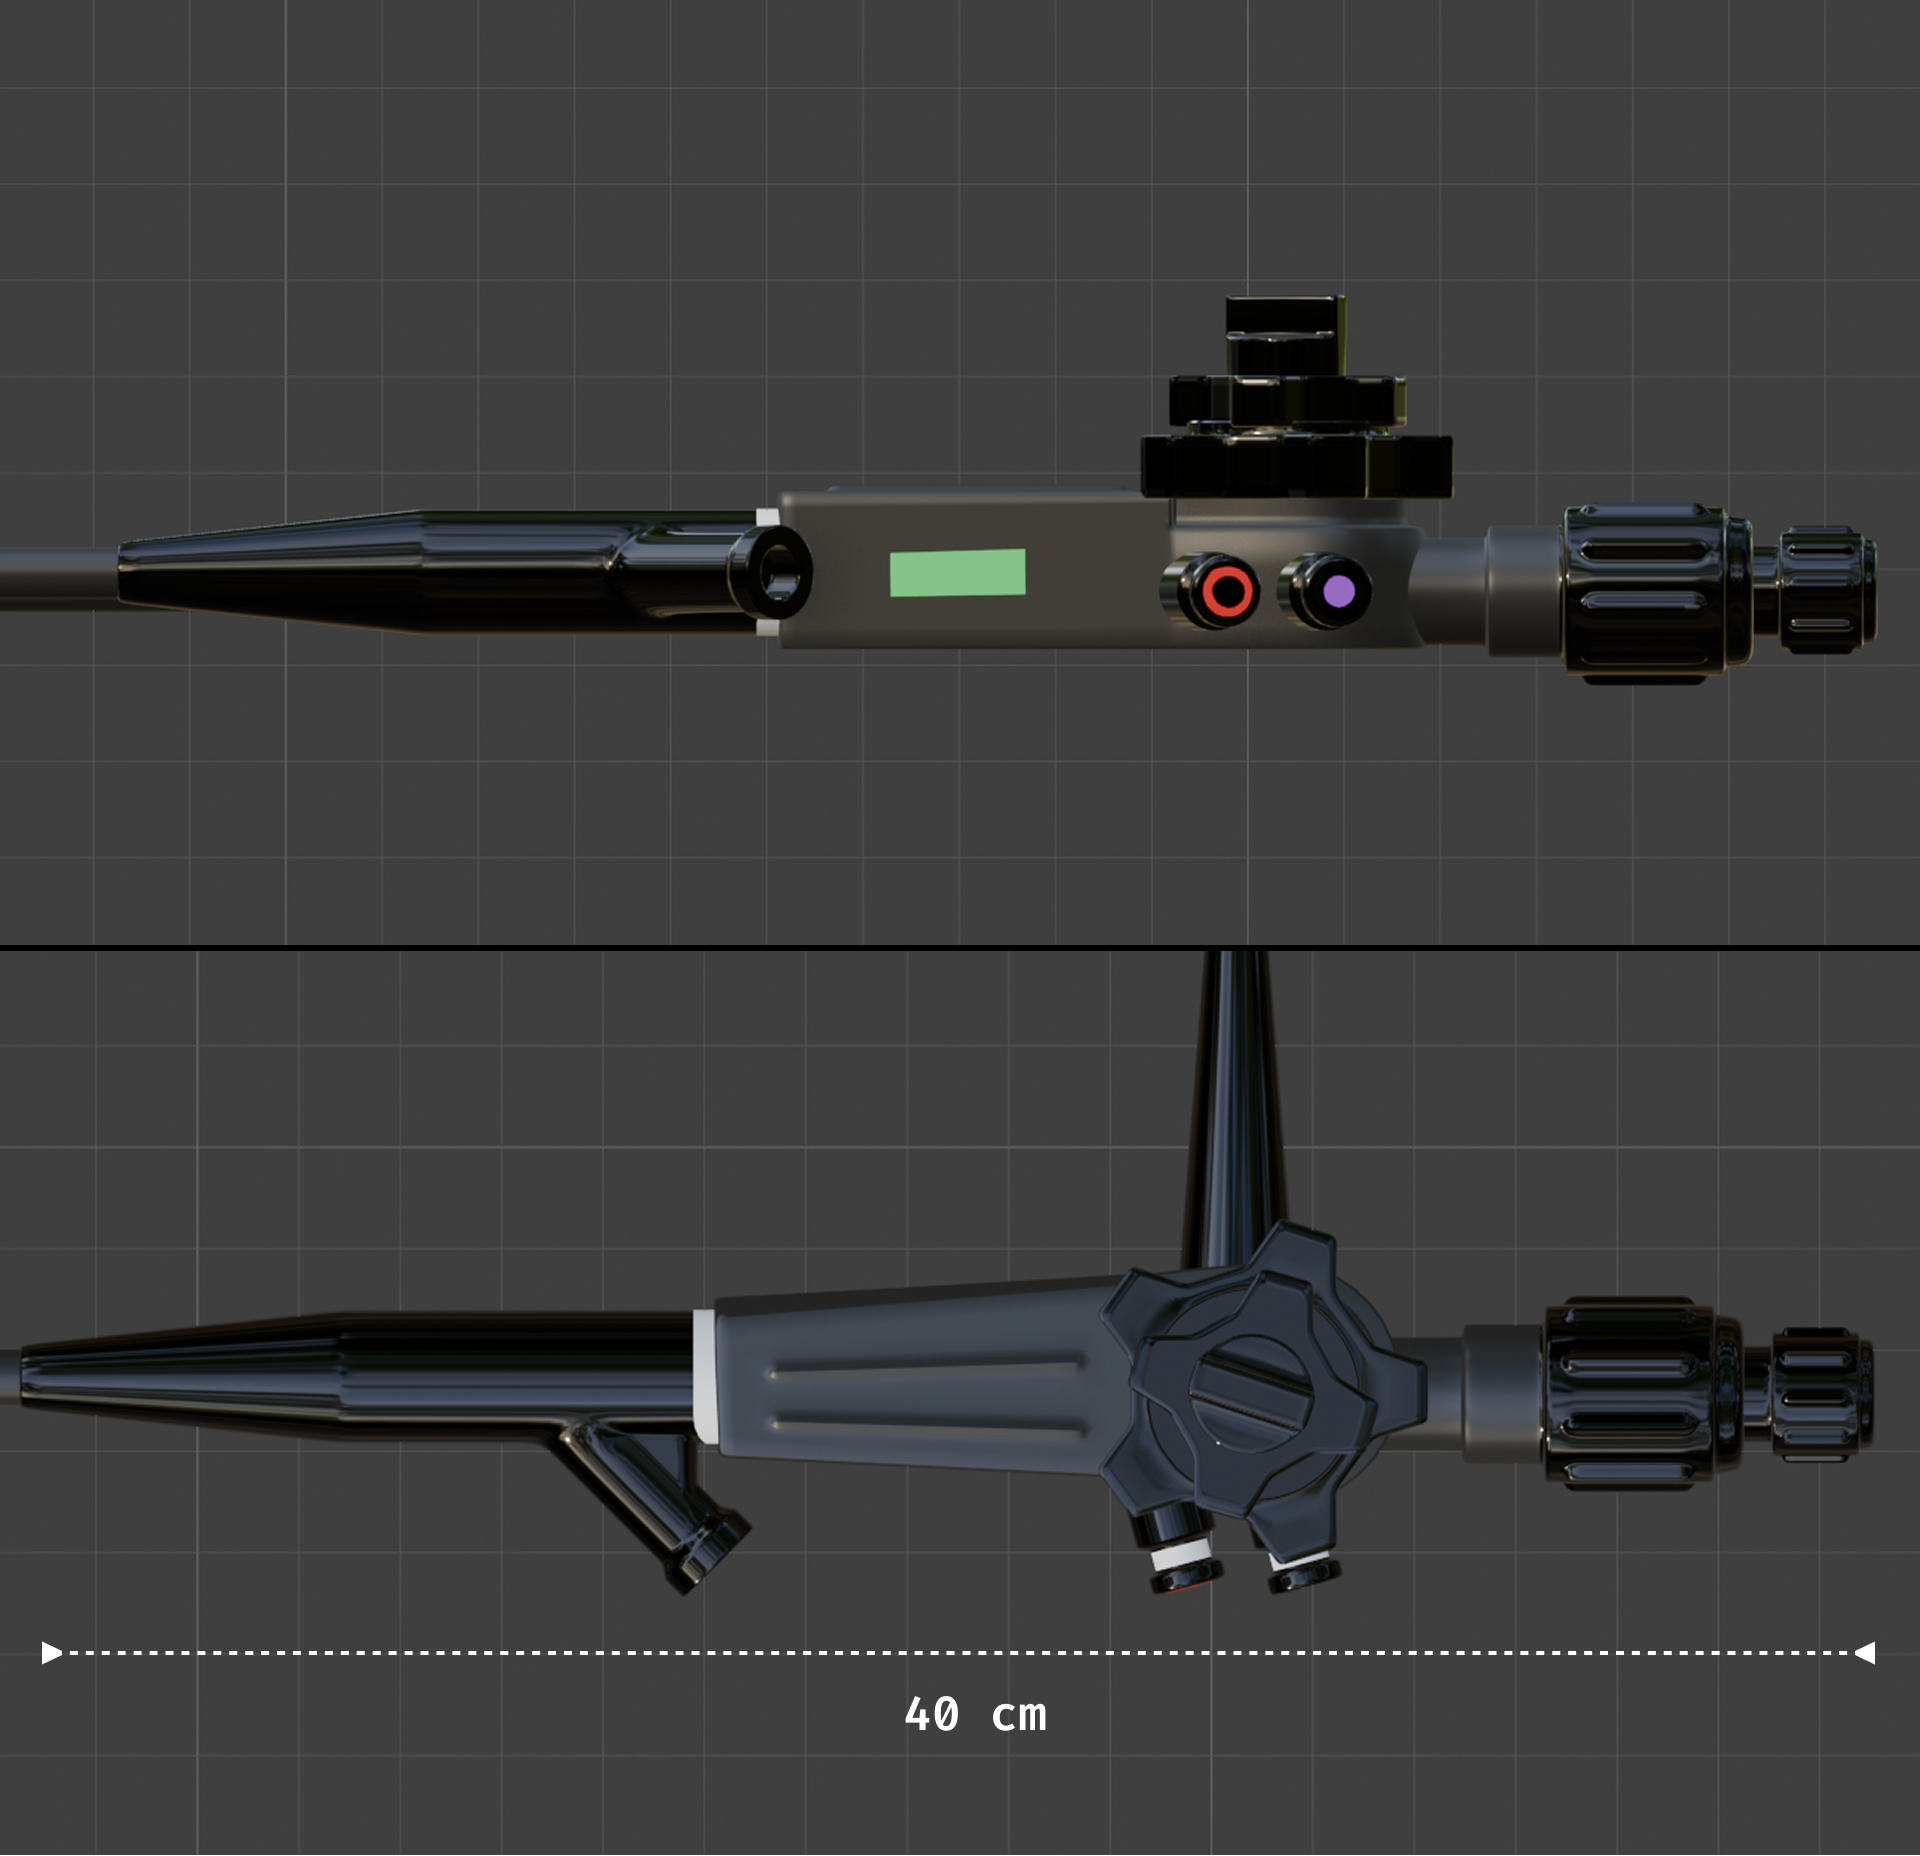
\includegraphics[width=0.6\linewidth,trim=0 0 0 2cm,clip]{assets/model-Endo Dim 2.png}
\caption{Close-up of the endoscope control head (approx. 40\,cm).}
\label{fig:model_endoscope_head}
\end{figure}


\paragraph{The insertion tube abstraction.}
Simulating a 170\,cm flexible tube via FEM would cripple frame rates. Instead, we \textbf{decouple forward translation from tip articulation}. The tip attaches to an \textbf{invisible kinematic pusher} gliding along a centerline spline at \textbf{2\,cm/s}. By forcing the forward momentum onto a set path, we successfully remove the messy problem of insertion dynamics (such as loop formation or colonic stretching) from the learning objective. This radical simplification ensures training remains computationally viable while still providing a rigorous testbed. Freed from soft-body physics, the agent focuses purely on \textbf{local visual steering}, preserving \textbf{hundreds of frames per second} for Deep RL!


% ==============================================================================
%                                 SNARE MODELING
% ==============================================================================
\clearpage
\subsection{Snare Modeling}

If the endoscope is the agent's eyes, the polypectomy snare is its fingers. Clinically, a snare is a braided metallic wire loop housed within a flexible plastic catheter. It advances through the instrument channel and expands to ensnare and slice the polyp. While conceptually simple, simulating a thin, flexible wire in a rigid-body physics engine is computationally expensive and notoriously difficult.

\begin{figure}[H]
\centering
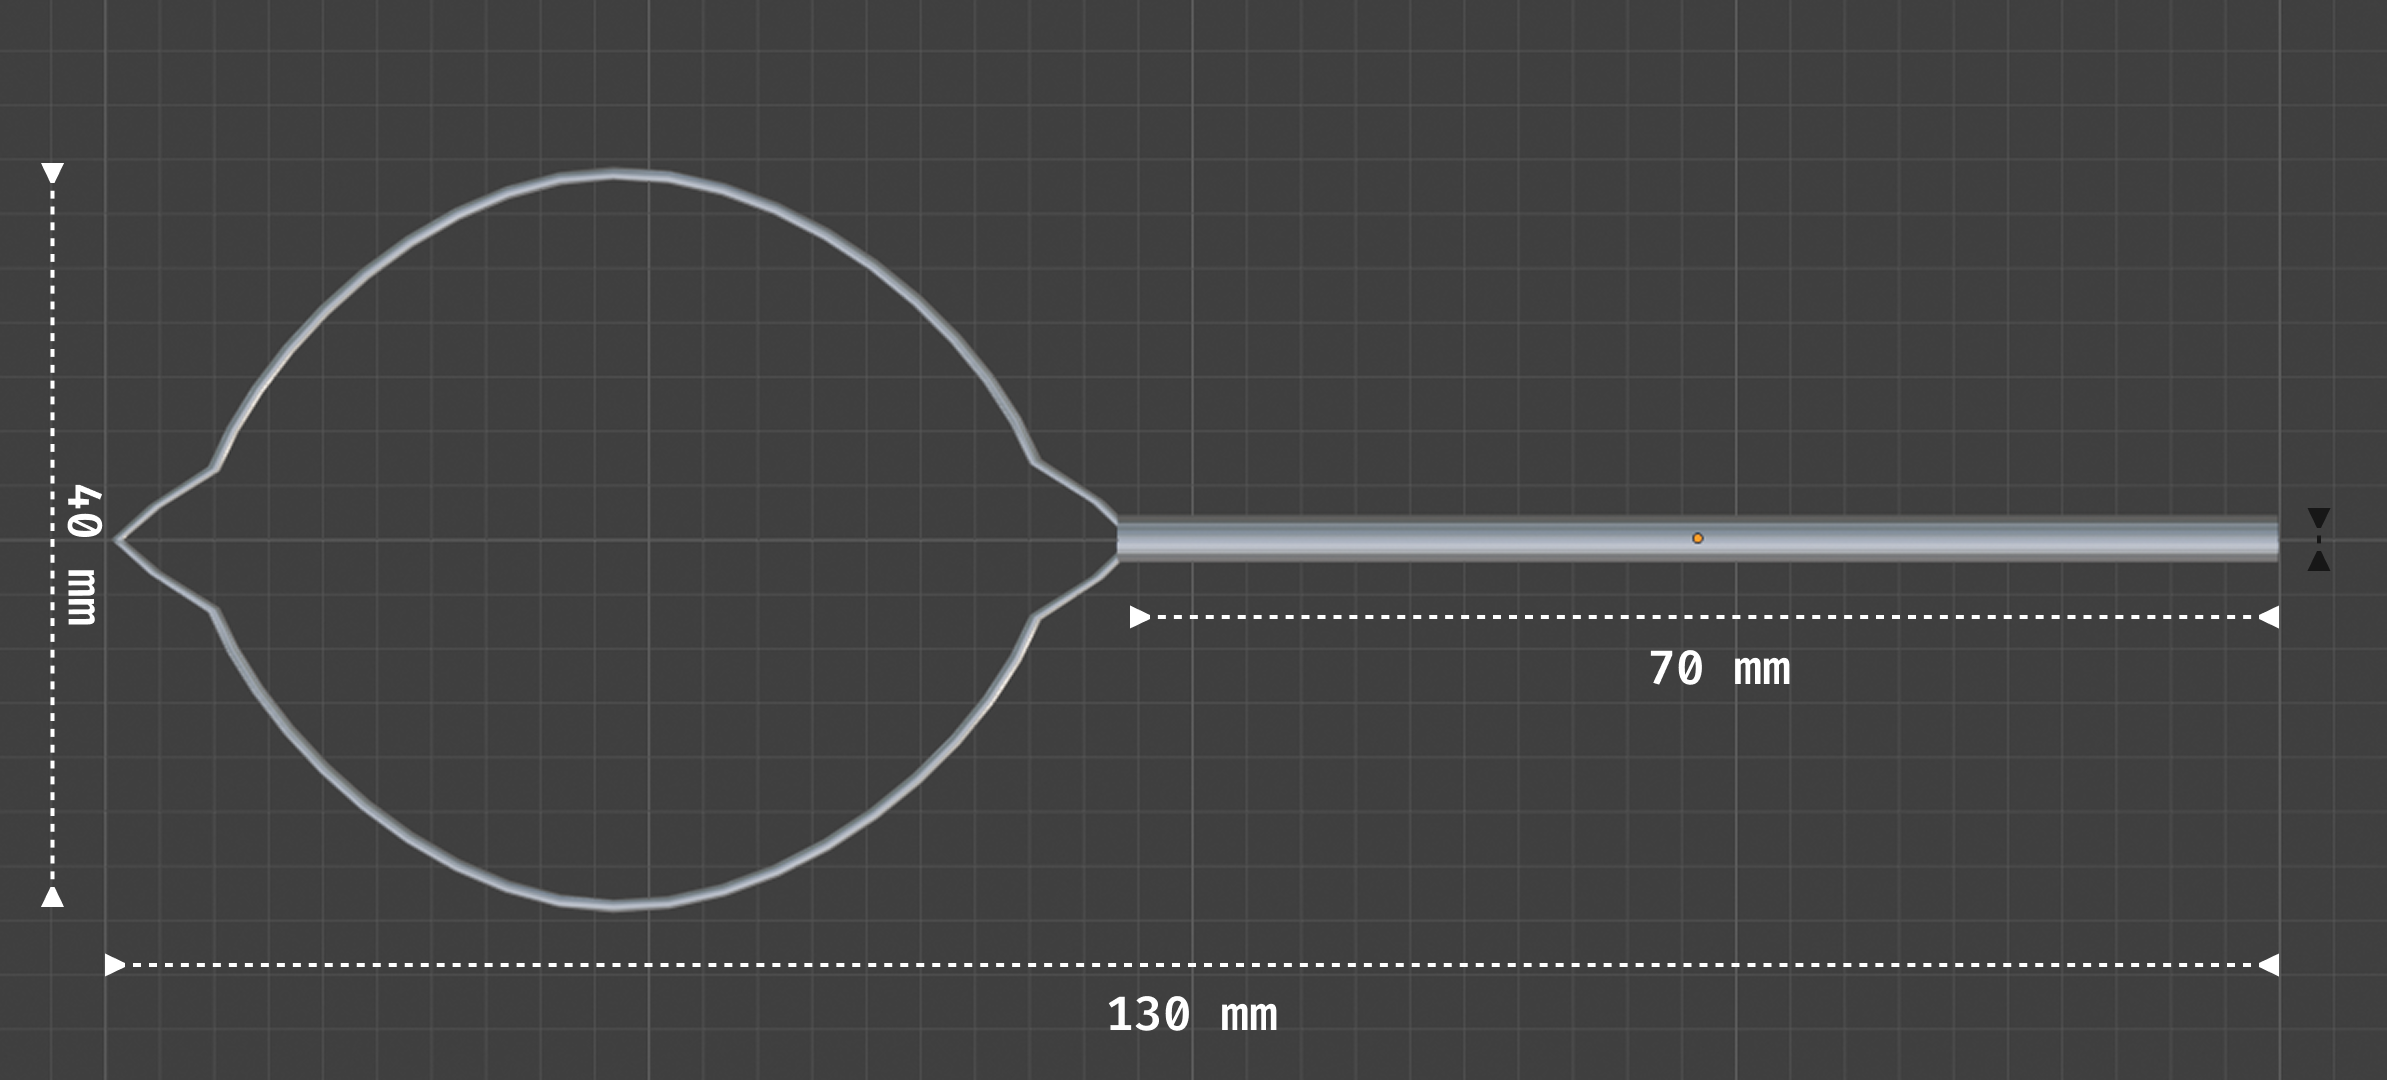
\includegraphics[width=0.8\linewidth]{assets/model-Snare Dimensions.png}
\caption{Dimensions of the snare model, detailing the catheter base and wire loop sizes.}
\label{fig:model_snare_dimensions}
\end{figure}

A standard catheter is 2.3 to 2.8\,mm thick, but the metallic wire loop is incredibly thin - usually just \textbf{0.30 to 0.47\,mm}! Yet, this loop can expand up to \textbf{35\,mm} in diameter. Because the wire's collision mesh is infinitesimally thin, high-velocity interactions frequently cause the engine to miss intersections entirely. This ``quantum tunneling'' or ``clipping'' means the wire passes straight through the polyp. Enforcing continuous collision detection prevents clipping but causes immense computational overhead and ``explosive'' physics glitches.

When continuous collision detection (CCD) is enforced on such fine geometry, physics engines like Unity attempt to calculate penetrations at every micro-step. If a 0.3\,mm wire even slightly overlaps a dense polyp mesh during a rapid rotational maneuver, the engine registers a deep penetration. To resolve this, it applies massive corrective penalty forces, often catapulting the snare across the virtual colon or causing it to vibrate violently. These unpredictable physical explosions immediately corrupt the reinforcement learning state space, feeding the agent catastrophic reward penalties that completely derail training. The agent essentially learns to fear moving the snare at all, leading to overly conservative policies that fail to capture the target. As a result, figuring out an alternative to traditional soft-body physics wasn't just about optimizing performance. It was actually a strict mathematical necessity if we wanted to keep the training environment stable.

To fix this, we abandoned soft-body dynamics for a \textbf{clever geometric abstraction}: a semi-rigid, articulated polygon structure. 
\begin{itemize}
\item \textbf{The Catheter Base:} A rigid cylindrical mesh sliding along the instrument channel.
\item \textbf{The Wire Loop:} A series of hinged, semi-rigid segments expanding or contracting procedurally.
\item \textbf{The Anchor Kinematics:} A proximal joint ensuring the snare inherits the camera's momentum.
\end{itemize}

Crucially, real snares do not just open and close; they are \textbf{fully rotatable}. We integrated this into the agent's action space, allowing complex maneuvers: extension, rotation, and loop actuation.

\begin{figure}[H]
\centering
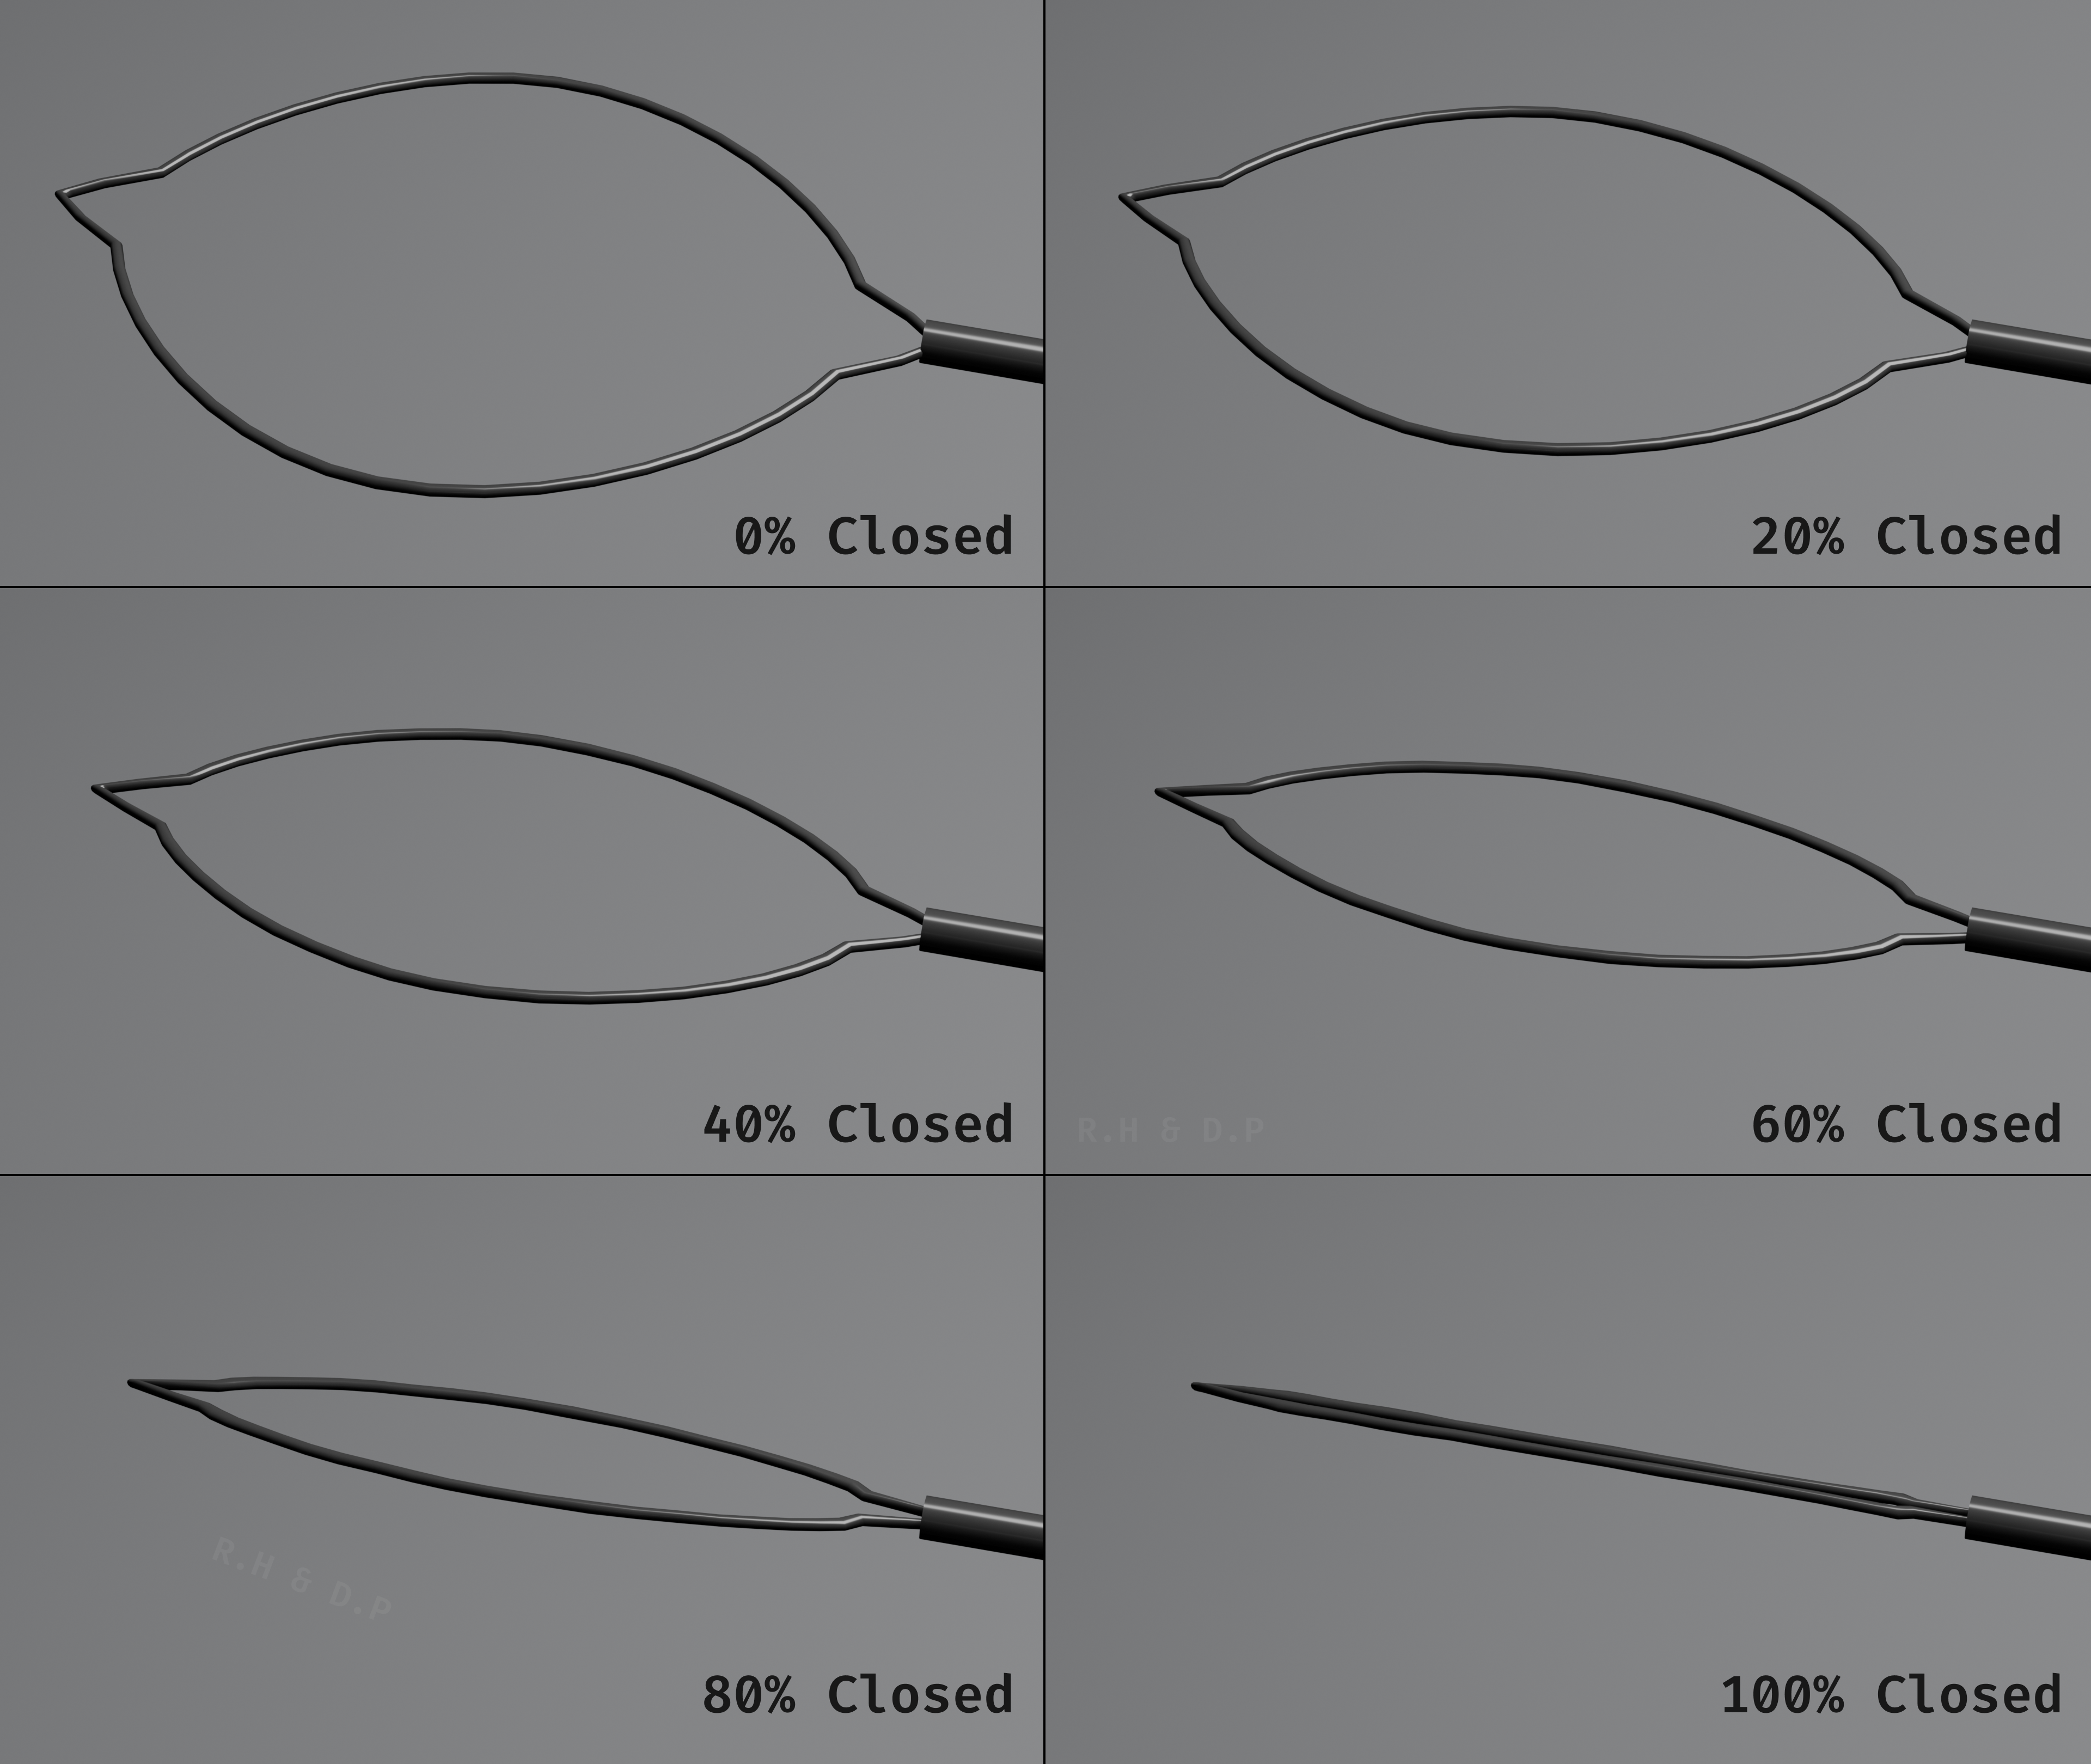
\includegraphics[width=0.8\linewidth]{assets/model-Snare Clamp Levels.png}
\caption{Different level of snare closure (0\% to 100\%)}
\label{fig:model_snare}
\end{figure}

The brilliance lies in the collision handling. Instead of an ultra-thin mesh, we attached overlapping invisible \textbf{``sphere colliders''} to the loop's hinged segments. As the cheapest mathematical shape to compute, spheres drastically reduce the load. When closing, these converging spheres form a shrinking cage. If the polyp is caught within this matrix, the system registers a ``grip.'' This provides deterministic behavior and eliminates soft-wire instability, letting the agent learn spatial timing without calculating complex mesh-deformations.




% ==============================================================================
%                                 COLON MODELING
% ==============================================================================
\clearpage
\subsection{Colon Modeling}

If the endoscope and snare are the agent's eyes and fingers, the colon is its \textit{world}. The human large intestine is a muscular, folded, \textbf{150\,cm-long tube} twisting through the abdomen. Its inner surface is corrugated by fleshy ridges called \textbf{haustra}, creating a massive total internal surface area of roughly \textbf{2\,000\,cm\textsuperscript{2}}.

Reproducing this topology is a \textbf{fundamental requirement} for Deep RL. Inside a smooth tunnel, moving forward produces no visual change. The \textbf{haustral folds} provide crucial \textbf{optic flow} - natural landmarks scrolling through peripheral vision that allow the CNN to estimate depth and speed. Figure~\ref{fig:model_colon_dim} shows our \textbf{110\,cm by 130\,cm} colon model.

\begin{figure}[H]
\centering
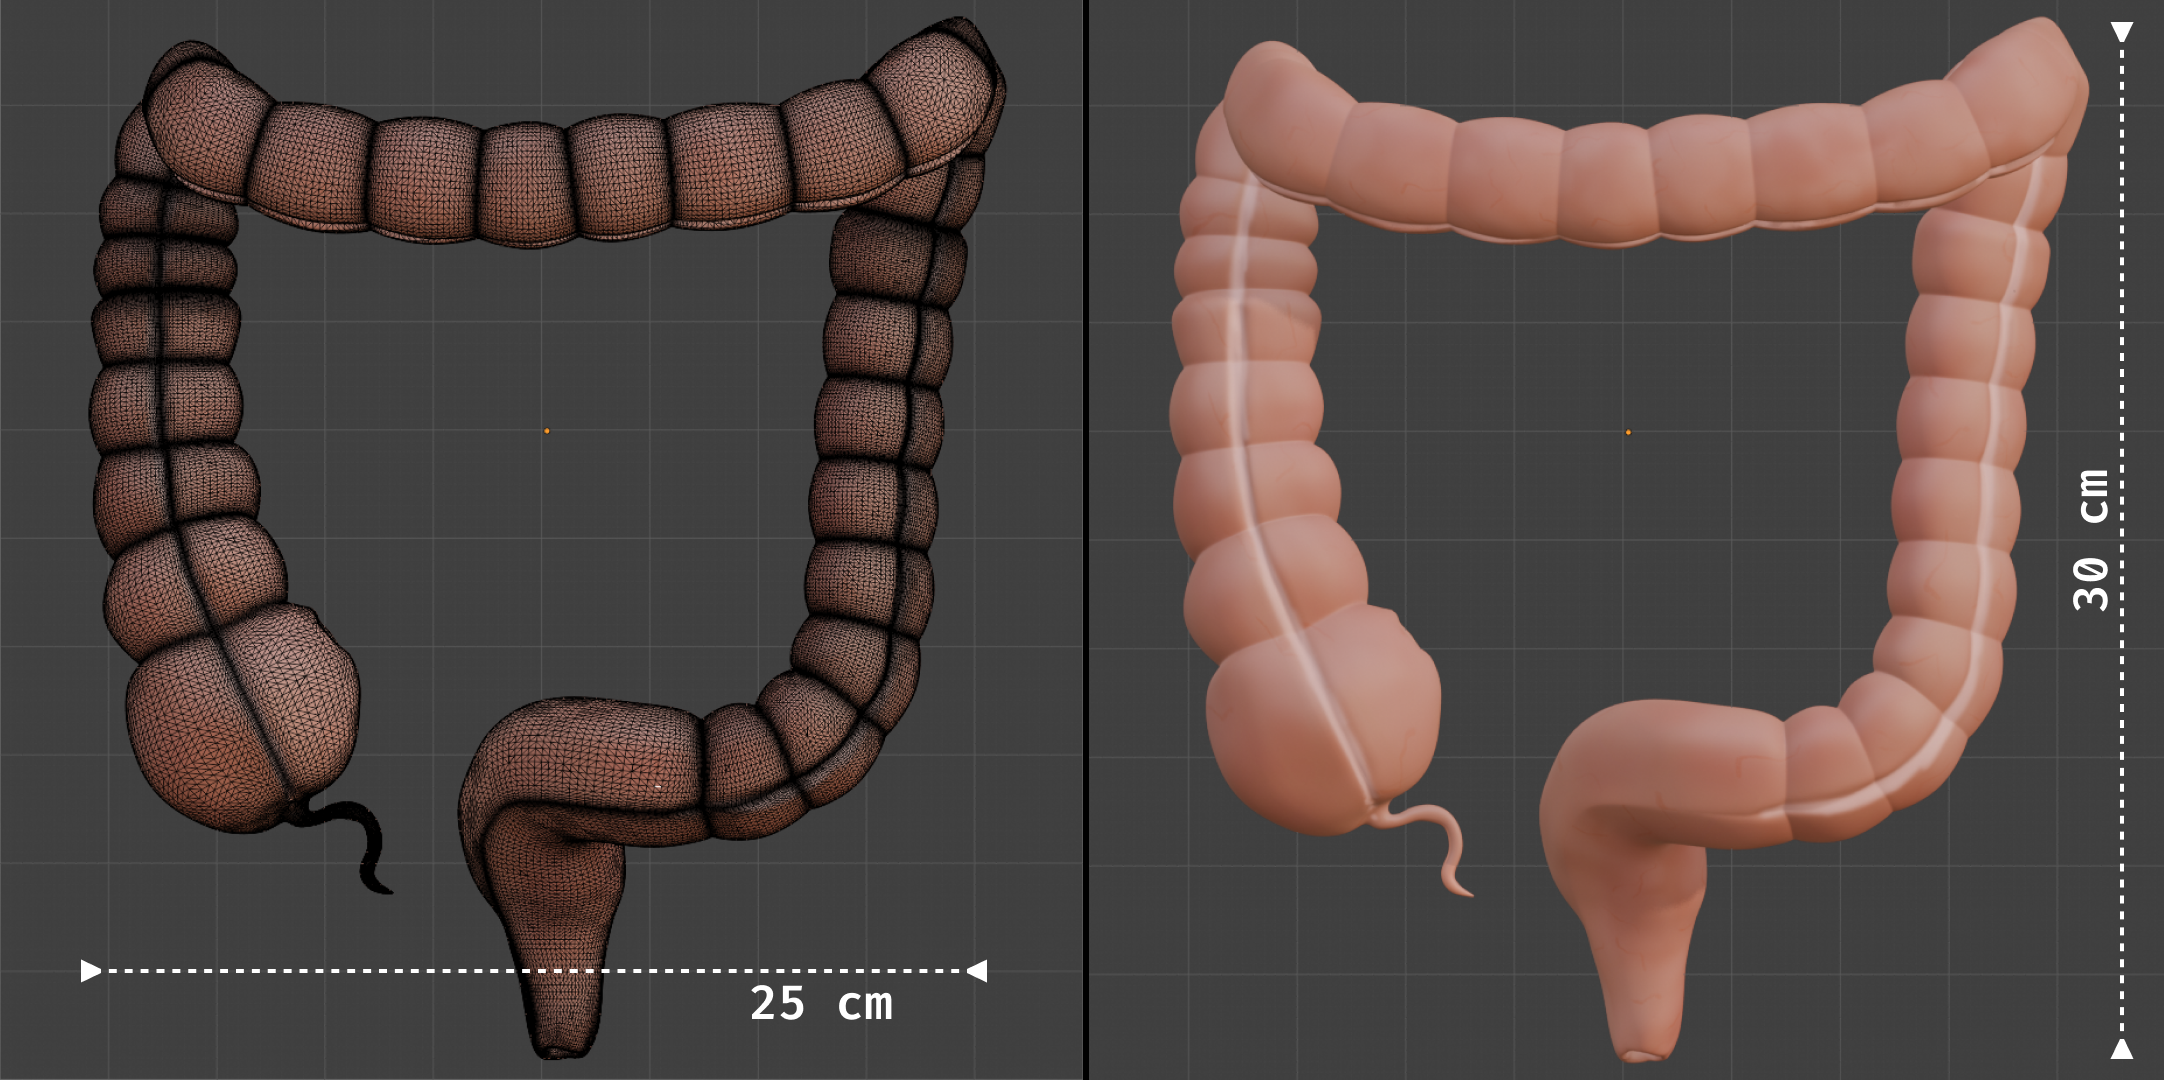
\includegraphics[width=0.8\linewidth]{assets/model-Colon Dim.png}
\caption{The colon 3D model in wireframe and shaded views, showing dimensions.}
\label{fig:model_colon_dim}
\end{figure}

\paragraph{Modular tile-set design.}
Instead of a single rigid 150\,cm mesh, we built a \textbf{modular tile-set} of colonic segments (curves, flexures, and strictures). Procedurally stringing these tiles together creates \textbf{diverse, randomized training tracks}, forcing the agent to actively steer rather than drift. 

The haustra were sculpted using \textbf{displacement modifiers} to create organic, asymmetrical folds. We kept mesh density moderate (\textbf{8\,000--12\,000 triangles} per segment) to maintain high frame rates for Deep RL training.

\paragraph{Texture, lighting, and the specular nightmare.}
The wet, vascular mucosal lining creates localized reflections called \textbf{specular highlights}. While gastroenterologists navigate these daily, they mask features and cause false-positive edges for CNNs. 

We built a custom \textbf{physically based rendering (PBR)} shader with a fleshy albedo map and high-smoothness specular map. We paired this with a rapidly decaying \textbf{point light} attached to the camera, mimicking a real endoscope. To further enhance realism, the shader incorporates a subtle \textbf{subsurface scattering} effect, simulating the way light penetrates and diffuses through biological tissue. Coupled with the point light's inverse-square attenuation, this setup ensures distant curves fade realistically into pitch black, forcing the agent to rely solely on proximal visual cues. Figure~\ref{fig:model_colon_insides} illustrates the resulting interior view.

\begin{figure}[H]
\centering
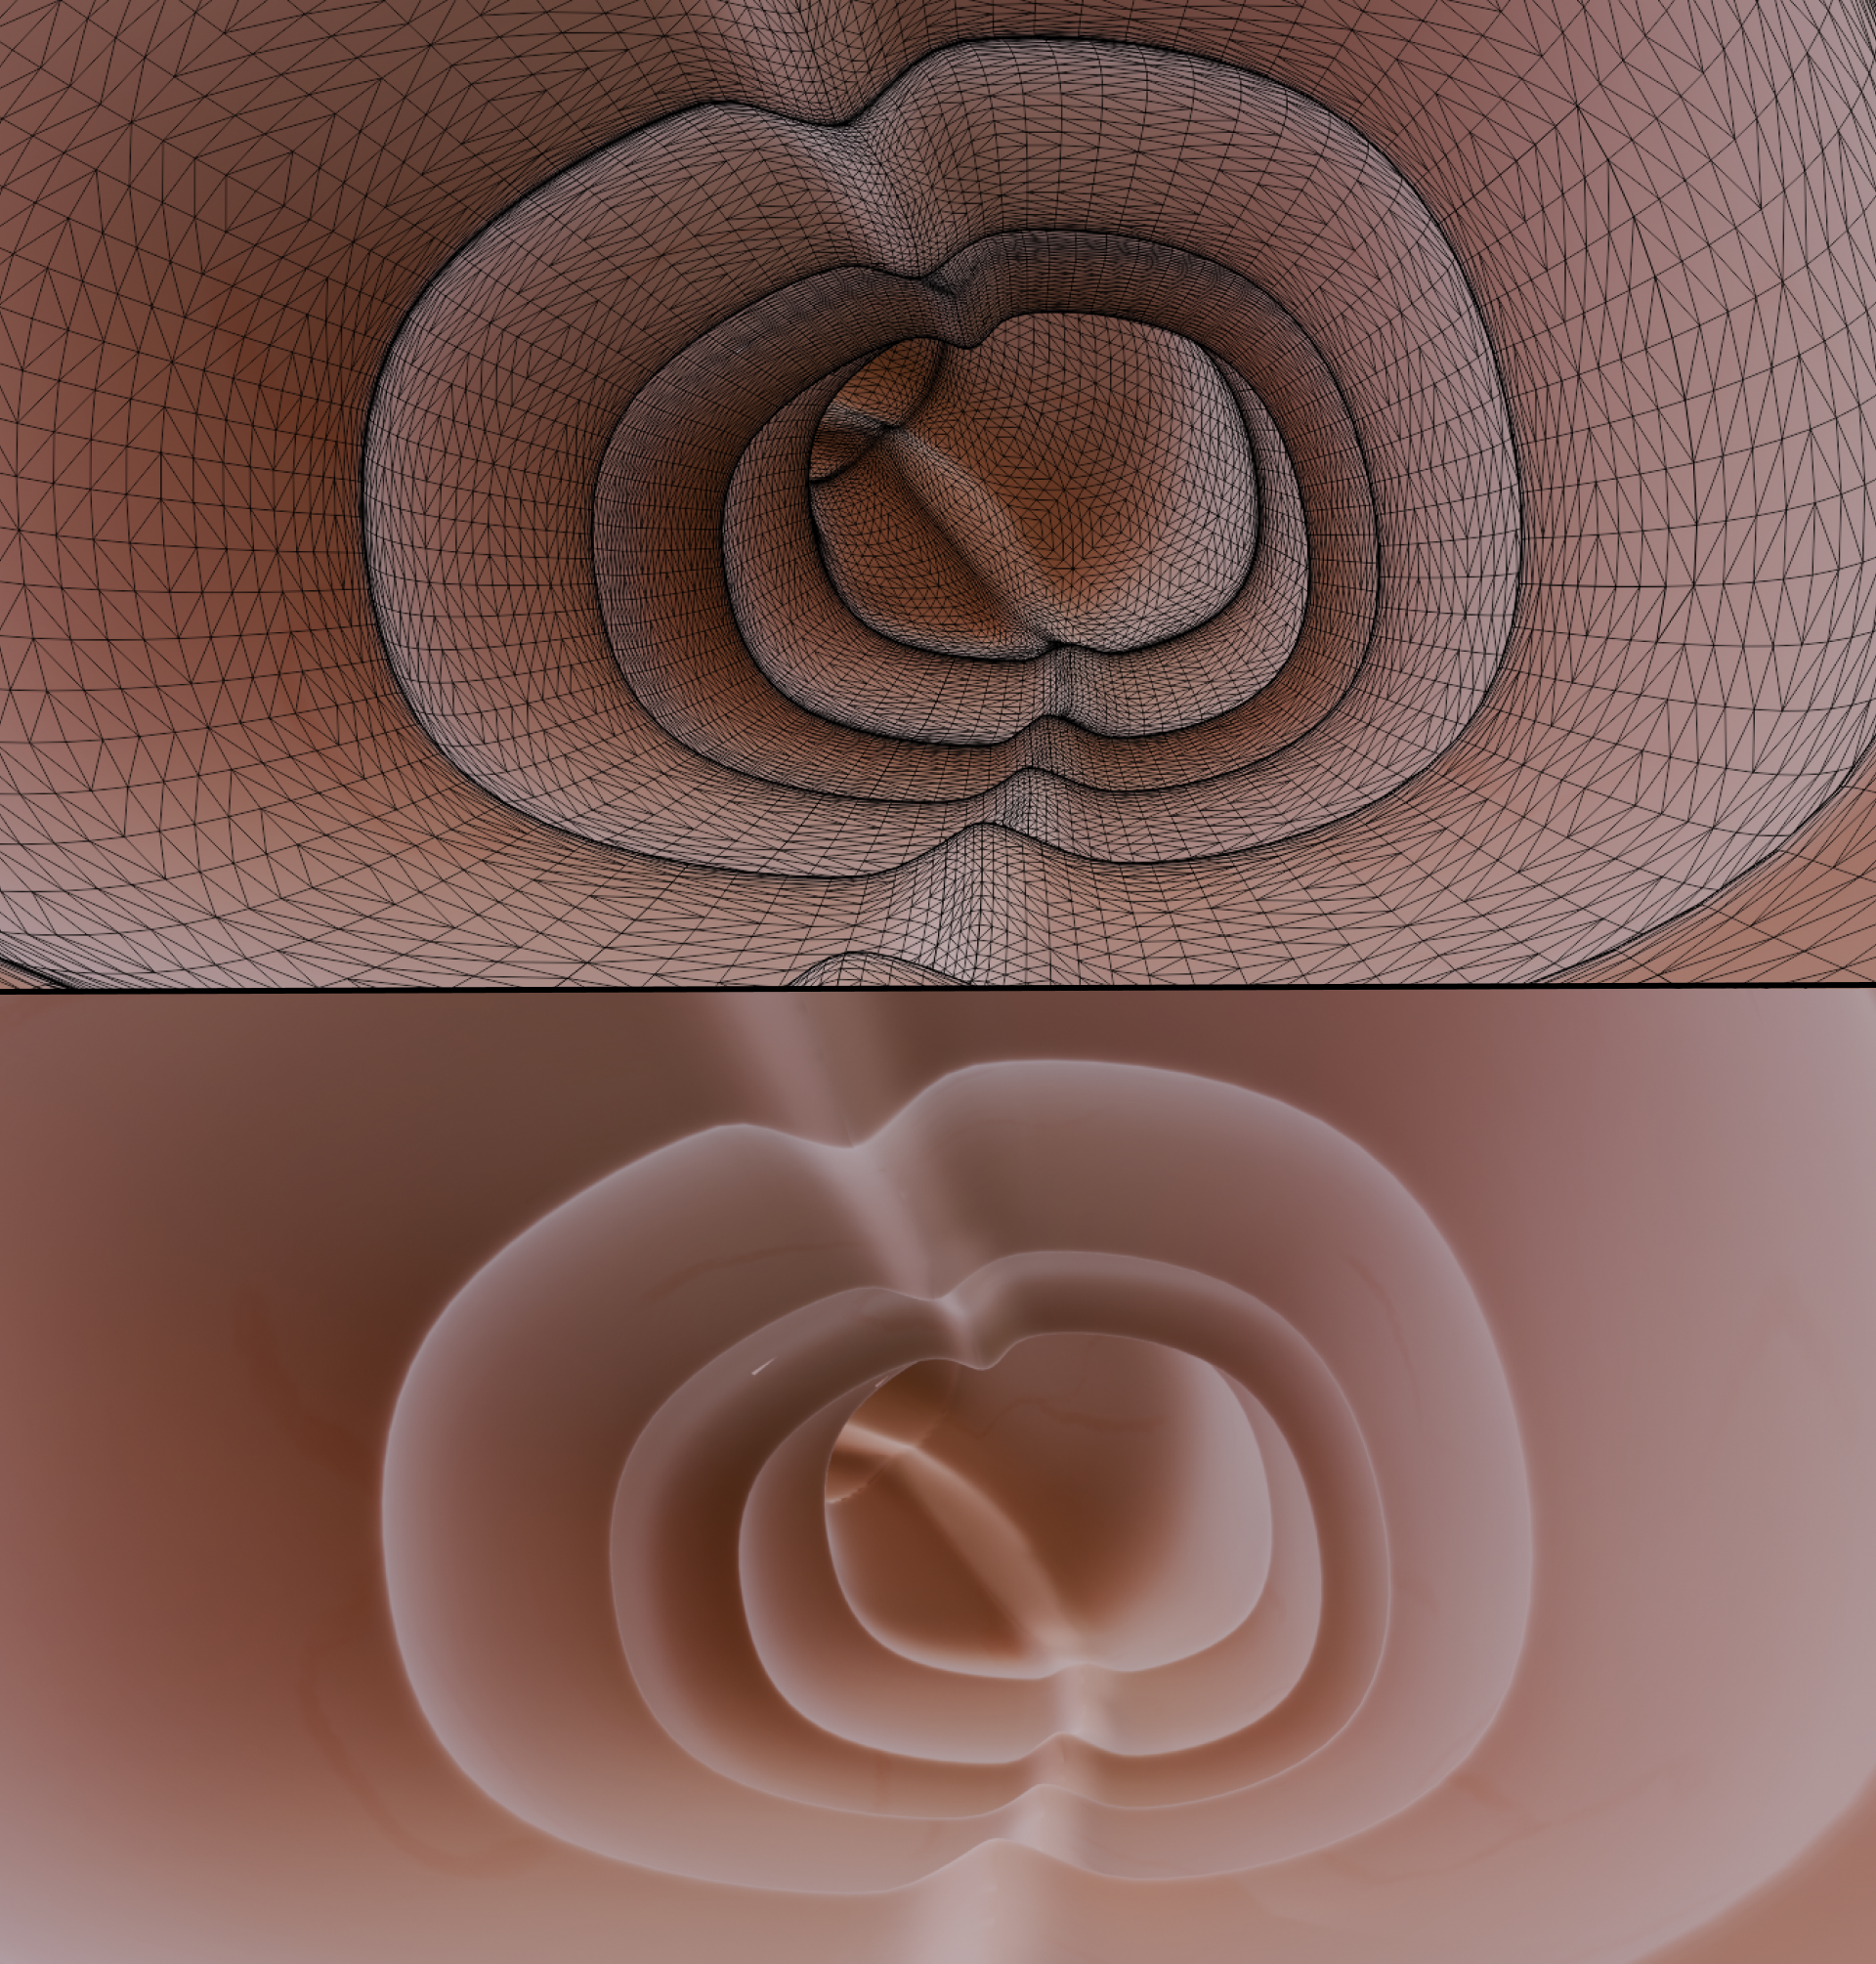
\includegraphics[width=0.6\linewidth]{assets/model-Colon Insides.png}
\caption{Interior view showing mesh topology and our custom PBR shader with dynamic point-light illumination.}
\label{fig:model_colon_insides}
\end{figure}

This environment is highly challenging: intense \textbf{specular highlights}, \textbf{dynamic shadows}, and \textbf{light attenuation} create harsh gradients. Because the light source is physically attached to the moving endoscope tip, the illumination field is inherently volatile. As the camera navigates the colon's tight curves, previously well-lit \textbf{haustral folds} are plunged into darkness while newly exposed \textbf{mucosal surfaces} flare with blinding reflections. This relentless \textbf{photometric variation} completely breaks traditional edge-detection techniques, which rely on stable lighting. By faithfully simulating these chaotic lighting conditions, we actively prevent the agent from memorizing brittle, \textbf{overfit visual patterns}. Instead, processing this relentless visual noise forces the \textbf{convolutional neural network (CNN)} to learn \textbf{robust, invariant features} that encode true \textbf{spatial depth} and \textbf{topological geometry}, rather than superficial pixel intensities. This ensures the resulting \textbf{navigation policy} is inherently resilient and mathematically primed for eventual \textbf{clinical deployment}.


% ==============================================================================
%                                 POLYP MODELING
% ==============================================================================
\clearpage
\subsection{Polyp Modeling}

The procedure's target is the \textbf{colorectal polyp}. The Paris classification defines \textbf{sessile} (flat) and \textbf{pedunculated} (stalked) polyps. We modeled a \textbf{pedunculated polyp} because they grow large (up to 30\,mm) and offer a specific snaring challenge: looping the head and cinching the stalk. Figure~\ref{fig:model_polyp_dim} shows our \textbf{30\,mm wide by 80\,mm tall} model.

\begin{figure}[H]
\centering
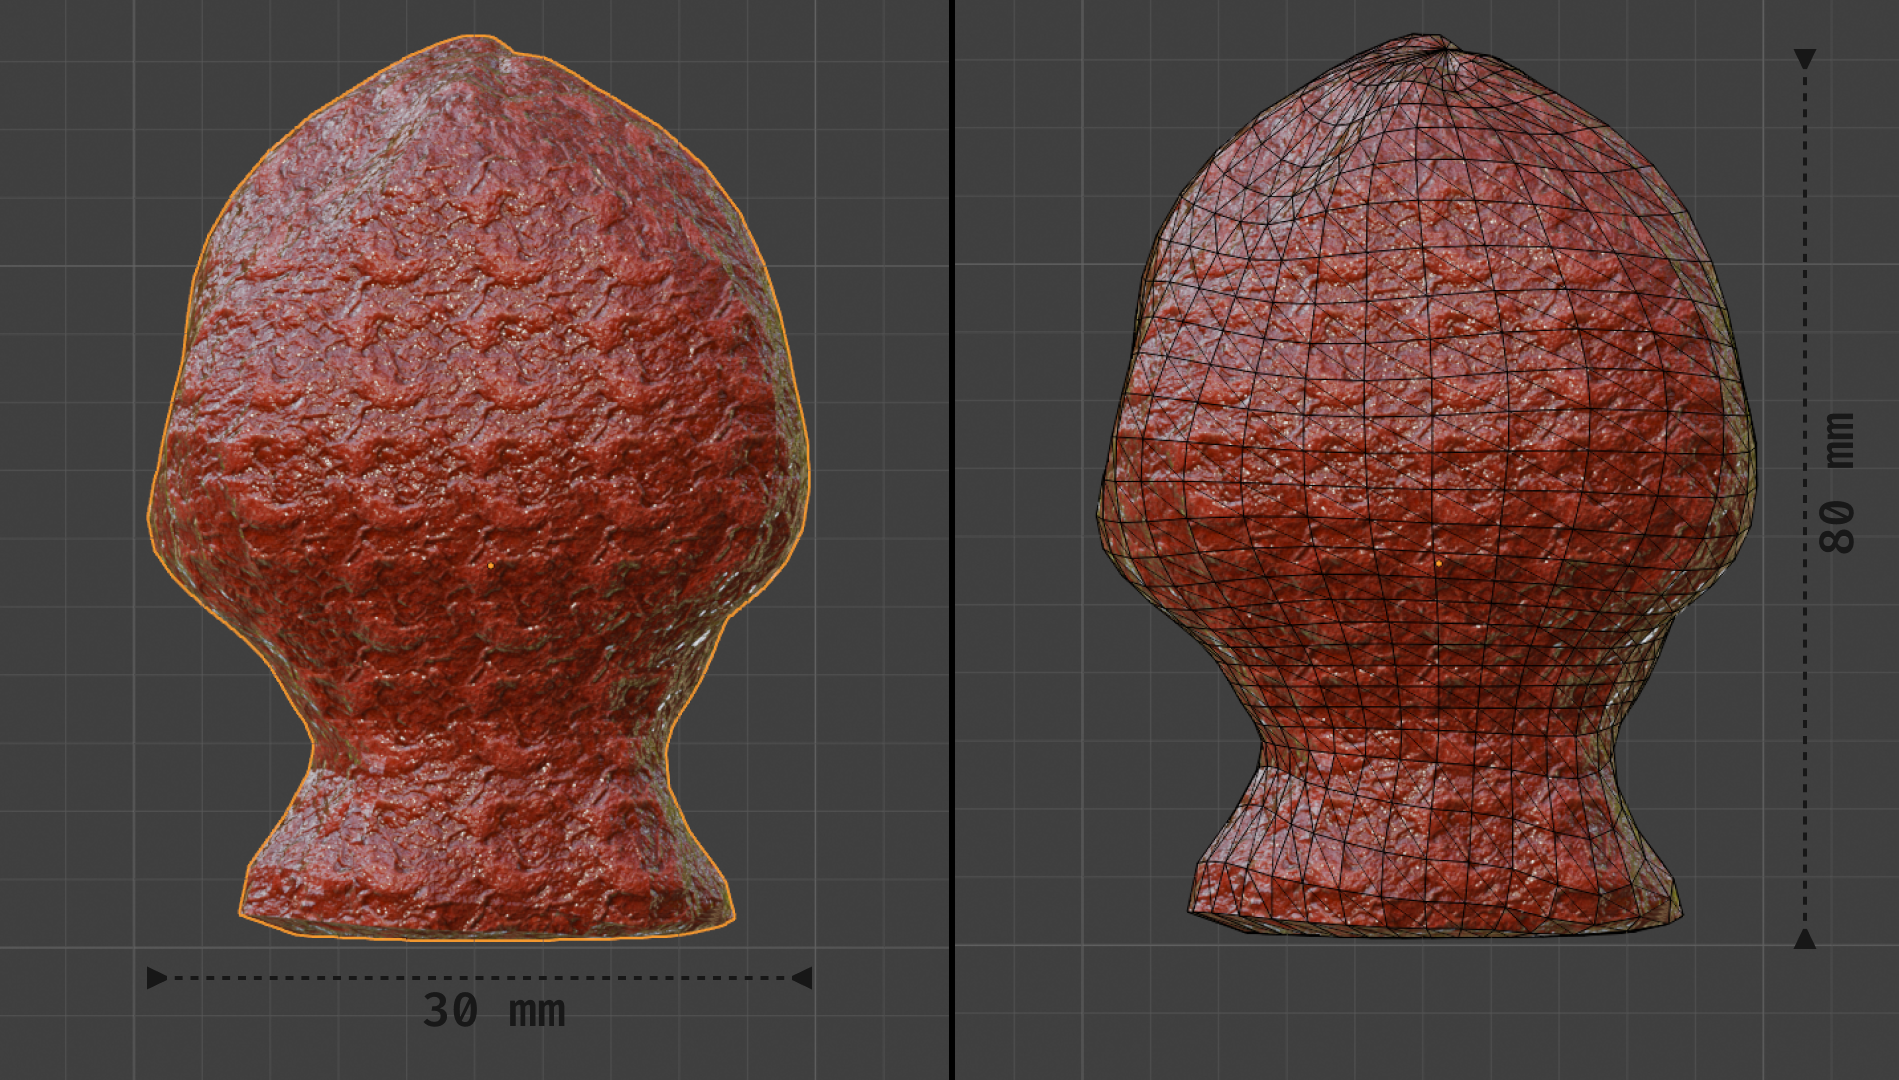
\includegraphics[width=0.6\linewidth]{assets/model-Polyp Dimensions.png}
\caption{Polyp 3D model (PBR material and wireframe), measuring 30\,mm by 80\,mm.}
\label{fig:model_polyp_dim}
\end{figure}

\paragraph{Visuals versus Physics.}
Visually, the polyp is a lumpy mushroom with a glossy, red-tinted PBR shader mimicking \textbf{hyperemia} (increased blood flow). Using this complex mesh for collision detection would be computationally wasteful and mathematically imprecise. Instead, we use a \textbf{dual-collider proxy system}.

\paragraph{The dual-collider proxy system.}
The physics engine ignores the visual mesh, relying entirely on two concentric \textbf{spherical triggers}:
\begin{itemize}
\item \textbf{The Core Sphere (Inner):} Located at the stalk's center. Perfect snare convergence around it yields the maximum reward.
\item \textbf{The Margin Sphere (Outer):} Defines the safe \textbf{resection margin}.
\end{itemize}

This translates clinical oncology into math. The golden rule is capturing a \textbf{1 to 2\,mm margin} of healthy tissue around the tumor to ensure a \textbf{curative resection}. 
